\begin{pastexam}[label={px:nchu-113-dsa-25}]{中興資工所甲組 113 學年度 申論題 PART 2 第 1 題}
（問答）

(5\%) Consider a Binary Search Tree (BST) with the following insertion sequence: [5, 3, 8, 2, 4, 7, 9]. What
is the result of a post-order traversal of this tree?
\end{pastexam}

\begin{pastsoln}
答案：$2, 4, 3, 7, 9, 8, 5$。

依序插入（資結書第~9.2~節）：$5$ 當根；$3 < 5$ 放左邊，$8 > 5$ 放右邊；$2$、$4$ 分別放 $3$ 的左、右；$7$、$9$
分別放 $8$ 的左、右。 得到一棵三層的完滿二元樹：
\begin{center}
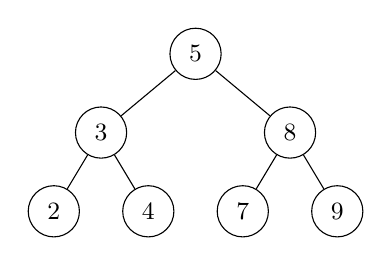
\begin{tikzpicture}[v/.style={circle,draw,minimum size=6.5mm,inner sep=1pt,font=\small},
  level distance=10mm, level 1/.style={sibling distance=24mm}, level 2/.style={sibling distance=12mm}]
\node[v] {5}
  child {node[v] {3} child {node[v] {2}} child {node[v] {4}}}
  child {node[v] {8} child {node[v] {7}} child {node[v] {9}}};
\end{tikzpicture}
\end{center}
後序（左、右、根）：先走左子樹 $3$ 的部分 $2, 4, 3$，再走右子樹 $8$ 的部分 $7, 9, 8$，最後根 $5$：
\[
2,\ 4,\ 3,\ 7,\ 9,\ 8,\ 5.
\]
\end{pastsoln}
